\section{Refinando petr\'oleo}
\subsection{Descripci\'on de la problem\'atica}

Dentro de una locaci\'on dada, se cuenta con \emph{n} pozos de extracci\'on de petr\'oleo. Como el petr\'oleo luego de ser extra\'ido debe ser refinado, se nos pide diagramar la construcci\'on de refiner\'ias y tuber\'ias para hacerlo posible.

Para armar esta red de refinamiento se podr\'an construir refiner\'ias, colocadas en cada pozo, y tuber\'ias que conectan los distintos pozos entre s\'i. Como todos los pozos deben tener un camino factible, para llegar a alguna planta procesadora, se les deber\'a colocar una planta de refinamiento en el mismo, o bien, armar un camino de tuber\'ias que lo conecte con una.
 
	Las refiner\'ias tienen un costo fijo, independiente del pozo donde se ubiquen, mientras que el costo de las tuber\'ias depende de los pozos que se quiera conectar. Adem\'as, contamos con la restricci\'on de que s\'olo se pueden construir tuber\'ias entre los pozos que nos son indicados. Todos estos datos nos son dados como par\'ametros de la funci\'on.\\

	Se desea escribir un algoritmo que de una distribuci\'on de refiner\'ias y tuber\'ias tal que todo pozo tenga acceso a una refiner\'ia y minimice el costo de la inversi\'on. Se debe indicar cu\'antas refiner\'ias construir y en qu\'e pozos, as\'i como tambi\'en cu\'antas tuber\'ias y entre que pozos.

	El algoritmo debe tener complejidad mejor que $O(n^3)$ siendo $n$ la cantidad de pozos de la zona.\\
\\

	A continuaci\'on citaremos una serie de ejemplos donde los modelamos como grafos, tal que los nodos son los pozos existentes y los ejes iniciales son las posibles conexiones entre ellos con un peso igual al costo de construir una tuber\'ia all\'i. En las soluciones, se preservan s\'olo los ejes donde construiremos una tuber\'ia y los nodos que sean amarillos representan pozos que contendr\'an una refiner\'ia en ellos.\\
	
	\newpage
	
	\underline{Ejemplo 1}: considerando un costo de construir una refiner\'ia igual a 7, contamos con la siguiente distribuci\'on de pozos y sus posibles conexiones:
	


  \begin{figure}[h!]
   \begin{center}
 	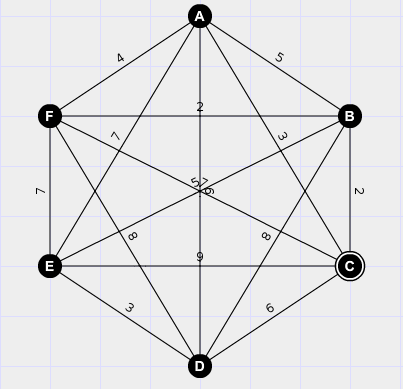
\includegraphics[scale=0.7]{imagenes/ej3/cliqueBIEN.png}
   \end{center}
 \end{figure}


La soluci\'on debe tener un costo total de 22 y es correcto devolver una distribuci\'on como la siguiente:
  \begin{figure}[h!]
   \begin{center}
 	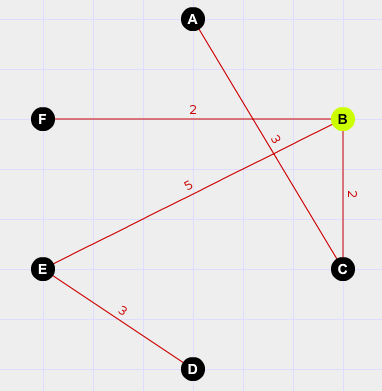
\includegraphics[scale=0.7]{imagenes/ej3/listoSIN.png}
   \end{center}
 \end{figure}

\newpage

	\underline{Ejemplo 2}: Consideramos otra distribuci\'on con un costo de construir una refiner\'ia igual a 6:
	
  \begin{figure}[h!]
   \begin{center}
 	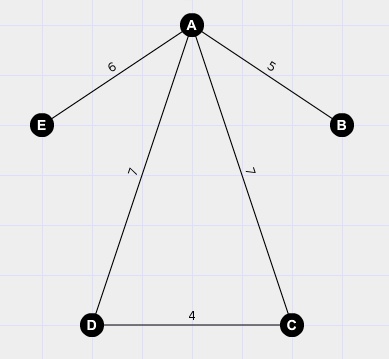
\includegraphics[scale=0.7]{imagenes/ej3/arbolCICLO.png}
   \end{center}
 \end{figure}
	
	La soluci\'on tendr\'a un costo total de 27, con la siguiente como una distribuci\'on v\'alida:

	
  \begin{figure}[h!]
   \begin{center}
 	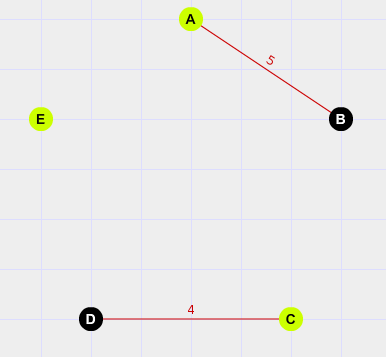
\includegraphics[scale=0.7]{imagenes/ej3/arbolLISTO.png}
   \end{center}
 \end{figure}

\newpage

\subsection{Resoluci\'on propuesta y justificaci\'on}

Dada la estructura del problema presentado, se opt\'o por modelar la situaci\'on mediante un grafo no dirigido. En este mismo, cada nodo presenta un pozo petrolero y los ejes indican la posibilidad de la construcci\'on de tuber\'ias. Es decir, dados dos nodos $e$ y $f$ del grafo, va a existir un eje $w=(e,f)$ si y solo si se puede construir una tuber\'ia entre $e$ y $f$. Adem\'as, cada eje va a contar con un peso que indica el costo de construcci\'on de su tuber\'ia.

Este grafo inicial se va a armar con los datos pasados por par\'ametro. En primera instancia, se guardan los ejes que se obtienen de la \emph{entrada standard} como una lista de adyacencia.\\

A partir de aqu\'i vamos a trabajar con un algoritmo particular sobre \emph{\'arboles generadores m\'inimos}: \textbf{algoritmo de Kruskal}.\\

El grafo obtenido hasta ahora puede tener desde $1$ hasta $n$ componentes conexas, para cada una de ellas vamos a formar su \'arbol generador m\'inimo. Esto nos asegurar\'a formar un \'arbol por componente tal que su peso total sea el m\'inimo de todos los \'arboles factibles. Al saber que los pesos de los ejes son todos positivos, contamos con que el \'unico camino resultante entre dos nodos va a ser el camino de menor costo de los caminos originales.\\

%LA WIKI PAPA
%Dado un grafo conexo y no dirigido, un árbol recubridor mínimo de ese grafo es un subgrafo que tiene que ser un árbol y contener todos los vértices del grafo inicial. Cada arista tiene asignado un peso proporcional entre ellos, que es un número representativo de algún objeto, distancia, etc.; y se usa para asignar un peso total al árbol recubridor mínimo computando la suma de todos los pesos de las aristas del árbol en cuestión. Un árbol recubridor mínimo o un árbol expandido mínimo es un árbol recubridor que pesa menos o igual que otros árboles recubridores. Todo grafo tiene un bosque recubridor mínimo.
% Si los pesos son positivos, el árbol recubridor mínimo es el subgrafo de menor costo posible conectando todos los vértices, ya que los subgrafos que contienen ciclos necesariamente tienen más peso total.

El algoritmo de Kruskal es un algoritmo goloso que est\'a implementado para grafos. Lo primero que realizamos fue ordenar los ejes que tenemos del grafo, por su peso en orden creciente. A continuaci\'on, se recorren los ejes secuencialmente y para cada uno se decide si debe permanecer o se debe quitar, de modo que si el eje actual no genera un ciclo (con los elegidos hasta esta instancia) permanece, en caso contrario se elimina.

Adem\'as, cuenta con una restricci\'on adicional. Cada eje que revisa va a permanecer s\'olo si su peso es menor al costo de construir una refiner\'ia. Esta nueva condici\'on, nos asegura que para cada pozo su camino para llegar a una refiner\'ia va a ser el m\'inimo. 

Consideremos el caso de $n=3$, donde contamos con los nodos: A, B y C con un costo de construir una refiner\'ia de \$10. A continuaci\'on, adjuntamos tres ejemplos donde se puede ver que la elecci\'on (entre insertar una tuber\'ia entre dos nodos o una refiner\'ia en cada uno) se condice con insertar una tuber\'ia s\'olo si su costo es menor al de construir una refiner\'ia.

  \begin{figure}[h!]
   \begin{center}
 	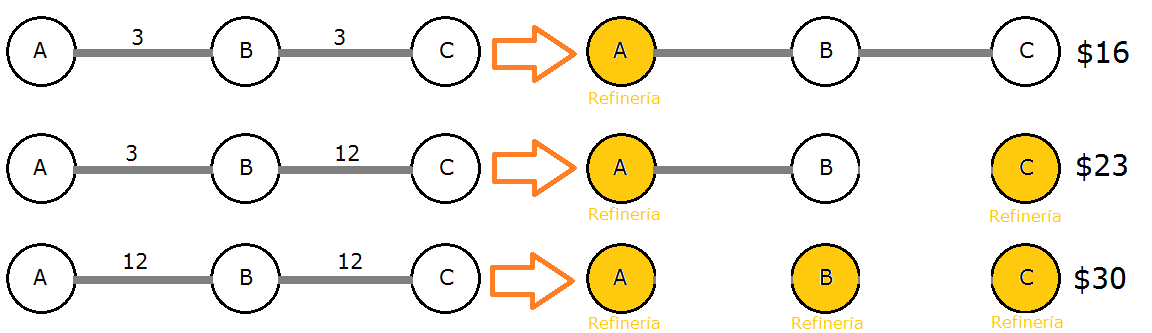
\includegraphics[scale=0.5]{imagenes/ej3/grafos.png}
   \end{center}
 \end{figure}


	Una vez que obtuvimos los ejes definitivos, nos queda simplemente contar cu\'antas refiner\'ias hay que colocar (una, por cada componente conexa -\'arbol- que formen los ejes seleccionados) y ubicarla en cualquier nodo de la componente.
	
	Llevar la cuenta de cu\'anto se lleva gastado es sumar los costos de cada tuber\'ia colocada m\'as la cantidad de refiner\'ias por su costo, y as\'i obtenemos el costo total.

\newpage
\subsection{An\'alisis de la complejidad}

Dados los datos ingresados como par\'ametros, contamos con el costo de construir una refiner\'ia y un grafo no dirigido de forma tal que la cantidad de nodos  est\'an numerados (arbitrariamente) de $0$ a $n-1$ y posee $m$ ejes. Tomamos como notaci\'on \emph{n = cantNodos} y \emph{m = cantEjes}.

Es importante destacar que la cantidad de ejes est\'a acotada por $O(n^2)$; ya que cada nodo, en el peor caso, puede conectarse con todos los nodos del grafo, excepto consigo mismo, es decir que para cada nodo, existen a lo sumo n-1 ejes que entran y salen del mismo.\\

El grafo que constru\'imos con los datos pasados como par\'ametro va a estar representado mediante una lista de adyacencia, la cual va a ser un vector de ejes. Esto presenta un costo de $O(m)$, como $m \leq n^2$ pertenece a $\mathbf{O(n^2)}$.\\

Luego, vamos a utilizar la estructura \emph{Union-Find} \footnote{Introduction to Algorithms (Third Edition) - Cormen, Leiserson, Rivest, Stein [2009], Unidad 21.} \footnote{Gregory C. Harfst and Edward M. Reingold. A potential-based amortized analysis of the
union-find data structure, 2000.	\label{paper}}. Esta estructura (adjuntada en el archivo \textit{UnionFind.h}) consiste de un vector capaz de almacenar diversos conjuntos disjuntos -cada uno con un \emph{Elemento Representante}-, la cual cuenta con los siguientes tres m\'etodos: \texttt{find_set(x)}, \texttt{union_set(x, y)} y \texttt{is_in(x, y)}. 

\texttt{find_set(x)} devuelve el elemento representante del conjunto al que pertenece \emph{x}.

\texttt{union_set(x, y)} une al conjunto que contiene a \emph{x} con el conjunto al que pertenece \emph{y}. 
 
\texttt{is_in(x, y)} devuelve true si \emph{x} est\'a en el mismo conjunto que \emph{y}, false en caso contrario. \\


El algoritmo de Kruskal se apoya en esta estructura. Nuestra funci\'on \texttt{generarArbolesMinimos} recibe como par\'ametros de entrada al vector de ejes totales, el costo de construir una refiner\'ia y la cantidad de pozos (n).


Como primer paso, ordena los ejes mediante el algoritmo  \href{http://www.cplusplus.com/reference/algorithm/sort/}{sort()} \footnote{http://www.cplusplus.com/reference/algorithm/sort/} de la librer\'ia Standard de \emph{C}, cuya complejidad es $O(m.log(m))$. Lo cual es equivalente a $O(n^2.log(n^2))$, por propiedades de logaritmo es $O(n^{2}2.log(n))$ y eliminando constantes es $\mathbf{O(n^2.log(n))}$. \\

%Crea un bosque m\'inimo que es un \emph{Union-Find}, Lo primero que hace es identificar los ejes donde es conveniente colocar una tuber\'ia para conectar dos pozos en vez de construir una refiner\'ia sobre ambos, aplicando el algoritmo de \textit{Kruskal}, apoyados sobre la estructura $Union-Find$.
%Luego por cada eje de los ejes obtenidos como par\'ametro de la funcion, si no forma un ciclo dentro de la componente conexa a la que pertenece, une ambos pozos, pero solo lo agrega al resultado si cuesta menos que poner una refiner\'ia. 

Luego, se recorren todos los ejes del vector obtenido como par\'ametro (\texttt{ejes}), ya ordenados. De modo que, primero nos ubicamos en el eje de menor costo, terminando el recorrido con el de mayor. Manejaremos un vector \texttt{res} y una estructura \emph{Union-Find} \texttt{(bosqueMinimo)}, que nos permitir\'an almacenar los ejes que sean candidatos v\'alidos para nuestra soluci\'on.

Al comienzo de la iteraci\'on, \texttt{res} estar\'a vac\'io y \texttt{(bosqueMinimo)} contendr\'a a todos los nodos, sin ninguna conexi\'on entre s\'i. Vamos a recorrer el vector \texttt{ejes} y por cada uno de ellos vamos a fijarnos si va a estar en la soluci\'on o no.

Esto implica verificar que, al agregarlos, no se forme un ciclo con los ejes ya iterados. Es decir, que s\'olo se unir\'an los dos nodos que une este eje dentro de su conjunto correspondiente en \texttt{(bosqueMinimo)}, si pertenecen a conjuntos distintos. Si es un eje v\'alido y su costo es menor al costo de construir una refiner\'ia, entonces lo agregamos a res.\\

%\textcolor{red}{Luego, se recorren todos los ejes del vector obtenido como par\'ametro (\texttt{ejes}), ya ordenados. De modo que, primero nos ubicamos en el eje de menor costo, terminando el recorrido con el de mayor. Contamos con un nuevo vector \texttt{res}, el cual va almacenar s\'olo los ejes que esten en el resultado, el cual comienza vac\'io. Para cada eje recorrido en \texttt{ejes}, se consulta si al insertarlo en \texttt{res} formar\'ia un ciclo con los que ya se encuentran en \'el. Si esta consulta es positiva, se saltea este eje; en caso contrario se inserta al vector \texttt{res} s\'olo si su costo es menor al costo de construir una refiner\'ia.}

%\textcolor{red}{Adem\'as vamos a contar con una estructura \emph{Union-Find} \texttt{(bosqueMinimo)}, la cual va a representar los conjuntos disjuntos que forman las componentes conexas del grafo. De modo que, al momento de insertar un nuevo eje a \texttt{res} dentro del ciclo tambi\'en se uniran los dos nodos que une este eje dentro de su conjunto correspondiente en \texttt{(bosqueMinimo)}.}\\

%\textcolor{blue}{Luego, se recorren todos los ejes del vector obtenido como par\'ametro (ejes), ya ordenados. De modo que, primero nos ubicamos en el eje de menor costo, terminando el recorrido con el de mayor. Manejaremos un vector \texttt{res} y una estructura \emph{Union-Find} \texttt{(bosqueMinimo)}, que nos permitir\'a saber si el eje es un candidato v\'alido para nuestro algoritmo. Esto implica verificar que no se forme un ciclo con los ejes ya iterados, es decir que solo se unir\'an los dos nodos que une este eje dentro de su conjunto correspondiente en \texttt{(bosqueMinimo)}, si pertencen a conjuntos distintos. Si es un eje v\'alido, entonces lo agregamos a res, pero s\'olo si su costo es menor al costo de construir una refiner\'ia.}\\

Este paso aprovecha la estructura de conjuntos disjuntos \textit{Union-Find}, para ver si dos conjuntos son disjuntos y eventualmente unirlos eficientemente. 

Dado que lo implementamos con las heur\'isticas de \textit{path compression} y \textit{union by rank}, la complejidad de $m$ operaciones \texttt{find_set} y \texttt{union-set} m\'as una llamada a \texttt{make_set} de complejidad $O(n)$, ejecutan en tiempo $O(m\alpha(n))$, donde $\alpha(n)$ es la inversa de\emph{ funci\'on de Ackerman}\textsuperscript{\ref{paper}}:

\begin{equation*}
\begin{array}{lll}
A(m,n) & = & (2\uparrow^{m-2}(n+3))-3 \\
\alpha(n) & = & min\{k \in N_0 : A(k,1) \geq n\}
\end{array}
\end{equation*}

	Algunos valores de la \emph{funci\'on de Ackerman} se presentan a continuaci\'on:

\begin{equation*}
\begin{array}{lll}
A(0,1) & = & 2 \\
A(1,1) & = & 3 \\
A(2,1) & = & 7 \\
A(3,1) & = & 2047 \\
A(4,1) & = & 10^{80}
\end{array}
\end{equation*}

	Como A crece excesivamente r\'apido, $\alpha$ crece excesivamente lento:

	\begin{equation*}
	\alpha(n) = 
	\begin{cases} 
		0  & \mbox{si } 0 \leq n \leq 2 \\
		1  & \mbox{si } n = 3 \\
		2  & \mbox{si } 4 \leq n \leq 7 \\
		3  & \mbox{si } 8 \leq n \leq 2047 \\
		4  & \mbox{si } 2048 \leq n \leq A(4,1) \\
	\end{cases}
	\end{equation*}

	Esto nos indica que para casi cualquier caso pr\'actico que empleemos (hasta $10^{80}$ nodos), $\alpha(n)$ ser\'a a lo sumo $4$. Por lo tanto, la complejidad de estas operaciones es $O(m)$ o lo que es lo mismo $\mathbf{O(n^2)}$.
	
	Tener en cuenta que, dentro del ciclo tambi\'en se ejecutan asignaciones y \href{http://www.cplusplus.com/reference/vector/vector/push_back/}{push\_back()} \footnote{http://www.cplusplus.com/reference/vector/vector/push_back/} en un vector pero estas operaciones cuentan con un costo $O(1)$ (amortizado en el caso de \texttt{push\_back}), lo cual es despreciable.\\

	Finalmente devuelve el vector resultante por copia, lo que suma, en el peor caso, $\mathbf{O(n)}$ dado que un \'arbol generador tiene a lo sumo $n-1$ ejes.\\

	Hasta este punto, la complejidad es la suma de las mencionadas:  $ O(n^2) + O(n^2.log(n)) + O(n^2) = \mathbf{O(n^2.log(n))}$.\\

	Resta hacer un recorrido lineal en los ejes del \'arbol generador m\'inimo que nos devolvi\'o el algoritmo de \textit{Kruskal}, armando un nuevo \textit{Union-Find} para distinguir cu\'ales son las componentes conexas resultantes. De esta manera, vamos a determinar 	qu\'e componentes necesitan una refiner\'ia (determinamos que el elemento representante de cada conjunto).
		
	 Esto tarda $\mathbf{O(n)}$ ya que, como se indic\'o anteriormente, a lo sumo son $n-1$ ejes.\\

	La cuenta final resulta $O(n) + O(n^2.log(n)) = \mathbf{O(n^2.log(n))}$, la cual es estrictamente mejor que $O(n^3)$ como se ped\'ia en el enunciado.


\newpage
\subsection{C\'odigo fuente}

	\begin{codesnippet}
	\begin{verbatim}
    class UnionFind {
    public:
        	UnionFind(int tamano);
        ~UnionFind();
        int find_set(int x);
        void union_set(int x, int y);
        bool is_in(int x, int y);

    private:
        vector<int> parent;
        vector<int> rank;
    };
	\end{verbatim}
	\end{codesnippet}

	\begin{codesnippet}
	\begin{verbatim}
    	UnionFind::UnionFind(int tamano){
        	parent = vector<int>(tamano);
        rank = vector<int>(tamano);
    //cada indice es su propio representante, su ranking es 0
        for (int i = 0; i < tamano; ++i) {
            parent[i] = i;
            rank[i] = 0;
        }
    }
	\end{verbatim}
	\end{codesnippet}

	\begin{codesnippet}
	\begin{verbatim}
    int UnionFind::find_set(int x) {
    //si es representante lo devuelvo, si no lo hago apuntar directamente al representante
    //para que llamadas consecutivas cuesten tiempo constante
        if(parent[x] != x)
            parent[x] = find_set(parent[x]);
        return parent[x];
    }
	\end{verbatim}
	\end{codesnippet}

	\begin{codesnippet}
	\begin{verbatim}
    void UnionFind::union_set(int x, int y) {
    //buscamos representantes de ambos elementos
    //requiere que no esten en el mismo conjunto
        int rx = find_set(x);
        int ry = find_set(y);
    //incluyo el de menor ranking en el de mayor para mantener balanceada la estructura
        if(rank[rx] < rank[ry]){
            parent[rx] = ry;
        }
        else{
            parent[ry] = rx;
            if(rank[ry] == rank[rx])
                rank[rx]++;
        }
    }
	\end{verbatim}
	\end{codesnippet}

	\begin{codesnippet}
	\begin{verbatim}
    bool UnionFind::is_in(int x, int y) {
        return find_set(x) == find_set(y);
    }
	\end{verbatim}
	\end{codesnippet}

	\begin{codesnippet}
	\begin{verbatim}
    struct eje {
        unsigned int pozoA;
        unsigned int pozoB;
        unsigned int costoTuberia;
        bool operator< (const eje& otro) const{
            return costoTuberia < otro.costoTuberia;
        }
    };
	\end{verbatim}
	\end{codesnippet}

	\begin{codesnippet}
	\begin{verbatim}
    int main(int argc, char const *argv[]){
        unsigned int pozos, cantConexiones, costoRefineria;
        unsigned int pozoA, pozoB, costoTuberia;
        cin >> pozos >> cantConexiones >> costoRefineria;
        vector<eje> ejes;
    //leemos la entrada, la almacenamos en ejes
        for (int i = 0; i < cantConexiones; ++i){
            cin >> pozoA >> pozoB >> costoTuberia;
            pozoA--;
            pozoB--;
            eje conex;
            conex.pozoA = pozoA;
            conex.pozoB = pozoB;
            conex.costoTuberia = costoTuberia;
            ejes.push_back(conex);
        }
    //aplicamos el algoritmo
        refinandoPetroleo(ejes, pozos, costoRefineria);
        return 0;
    }
	\end{verbatim}
	\end{codesnippet}

	\begin{codesnippet}
	\begin{verbatim}
    int refinandoPetroleo(vector<eje>& ejes, int cantPozos, int costoRefineria){
    //generamos los arboles minimos para cada componente conexa, 
    //en realidad solo los ejes que cuesten menos que poner refinerias
        vector<eje> conexionesMinimas = generarArbolesMinimos(ejes, costoRefineria, cantPozos);
        UnionFind conexos(cantPozos);
        int costoTotal = 0, cantRef = 0;
    //armamos un union-find para identificar componentes triviales, en las demas solo hara falta 
    //poner una refineria en el representante de la componente pues los tubos son mas baratos 
    //para unir los distintos pozos
        for (int i = 0; i < conexionesMinimas.size(); ++i) {
            conexos.union_set(conexionesMinimas[i].pozoA, conexionesMinimas[i].pozoB);
            costoTotal += conexionesMinimas[i].costoTuberia;
        }
    //en las componentes triviales van refinerias
        vector<bool> refinerias(cantPozos);
        for (int i = 0; i < cantPozos; ++i) {
            if(conexos.find_set(i) == i){
                refinerias[i] = true;
                costoTotal += costoRefineria;
                cantRef += 1;
            }
        }
    //cout pedido
        cout << costoTotal << " " << cantRef << " " << conexionesMinimas.size() << endl;
        for (int i = 0; i < refinerias.size(); ++i) {
            if(refinerias[i])
                cout << i+1 << " ";
            }
        cout << endl;
        for (int i = 0; i < conexionesMinimas.size(); ++i) {
            cout << conexionesMinimas[i].pozoA+1 << " " << conexionesMinimas[i].pozoB+1 << endl;
        }
        return costoTotal;
    }
	\end{verbatim}
	\end{codesnippet}

	\begin{codesnippet}
	\begin{verbatim}
    vector<eje> generarArbolesMinimos(vector<eje>& ejes, int costoRefineria, int cantPozos){
        UnionFind bosqueMinimo(cantPozos);
        vector<eje> res;
    //ordenamos los ejes segun su costo para obtener en tiempo constante, los menores
        sort(ejes.begin(), ejes.end());
        for (int i = 0; i < ejes.size(); ++i) {
    //si agregar el eje no forma ciclo
        if(!bosqueMinimo.is_in(ejes[i].pozoA,ejes[i].pozoB)){
    //lo uno y si cuesta menos que poner una refineria, lo agrego a res
            bosqueMinimo.union_set(ejes[i].pozoA, ejes[i].pozoB);
                if(ejes[i].costoTuberia < costoRefineria){
                    eje conex;
                    conex.pozoA = ejes[i].pozoA;
                    conex.pozoB = ejes[i].pozoB;
                    conex.costoTuberia = ejes[i].costoTuberia;
                    res.push_back(conex);
                }
            }
        }
        return res;
    }
	\end{verbatim}
	\end{codesnippet}

\newpage
\subsection{Experimentaci\'on}
\subsubsection{Constrastaci\'on Emp\'irica de la complejidad}
	Para llevar a cabo esta experimentaci\'on, consideramos el peor caso posible de cantidad de ejes del grafo, es decir que habr\'a exactamente $n.(n-1)$ ejes (cada nodo puede conectarse con cualquier nodo del grafo, excepto consigo mismo), variando la cantidad de nodos.\\


	Armamos un script que gener\'o estas instancias, toma como par\'ametro la cantidad de pozos, y el costo de la refiner\'ia, las conexiones no, porque quer\'iamos un grafo completo, este valor ser\'a $n.(n-1)$. El mismo escribe un archivo con el formato de la entrada standard, donde a cada eje le asigna un peso random entre 0 y 2\texttt{*}costoRefiner\'ia.\textcolor{red}{El archivo se adjunta en... y se llama ...}\\

	Los tiempos de ejecuci\'on para cada n (cantidad de nodos) fueron los siguientes:

	\begin{table}[htb]
	\centering
	\begin{tabular}[c]{|l|l|}

		\hline
n & Tiempo en segundos\\
		\hline
50	&	0.0005254864\\
		\hline
100	&	0.002332719\\
		\hline
150	&	0.0059328642\\
		\hline
200	&	0.01065945\\
		\hline
250	&	0.0178728144\\
		\hline
300	&	0.0277215188\\
		\hline
350	&	0.0373807766\\
		\hline
400	&	0.0487278266\\
		\hline
450	&	0.0661190683\\
		\hline
500	&	0.0807527896\\
		\hline
550	&	0.0978193478\\
		\hline
600	&	0.126140013\\
		\hline
650	&	0.146378511\\
		\hline
700	&	0.168847877\\
		\hline
750	&	0.192539493\\
		\hline
800	&	0.219705288\\
		\hline
850	&	0.267457097\\
		\hline
900	&	0.301437881\\
		\hline
950	&	0.332602623\\
		\hline
1000	&	0.366929358\\
		\hline

	\end{tabular}
	%\caption{Tabla muy sencilla.}
	%\label{tabla:n.png}
	\end{table}

  \begin{figure}[h!]
   \begin{center}
 	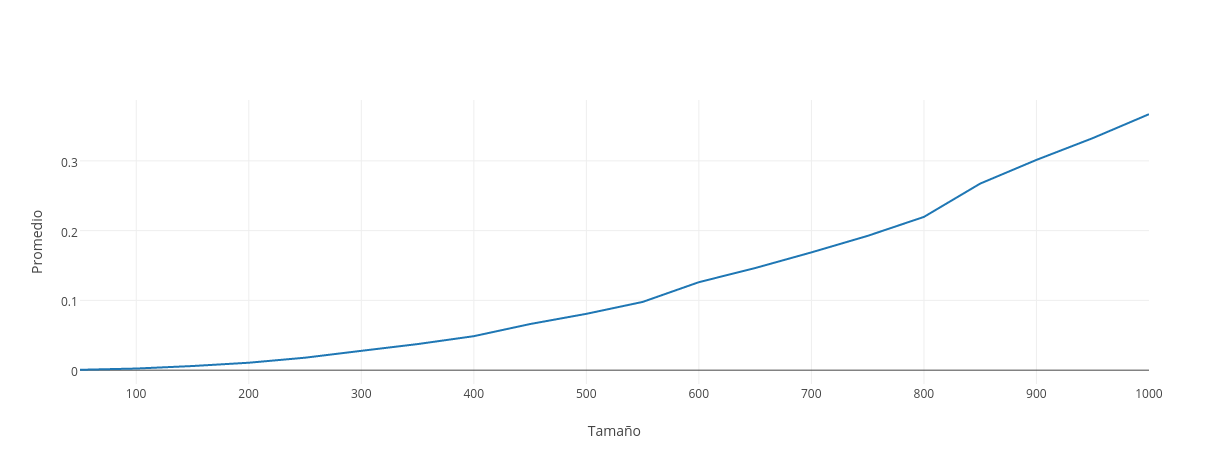
\includegraphics[scale=0.4]{imagenes/ej3/n2logn.png}
% 	\caption{}
% 	\label{n.png}
   \end{center}
 \end{figure}

 \newpage

	Dado que la Cota de Complejidad planteada te\'oricamente es de $O(n^2.log(n))$, era esperable que la curva sea una par\'abola creciente.

	A simple vista, no se puede apreciar si la relaci\'on que tienen respecto de tama\~no/tiempo es efectivamente la que buscamos (pues casi todas las curvas polinomiales tienen gr\'aficos similares). Por este motivo, como siguiente paso decidimos comenzar a linealizar los tiempos, dividiendo a cada uno por $log(n)$.

   \begin{figure}[h!]
   \begin{center}
 	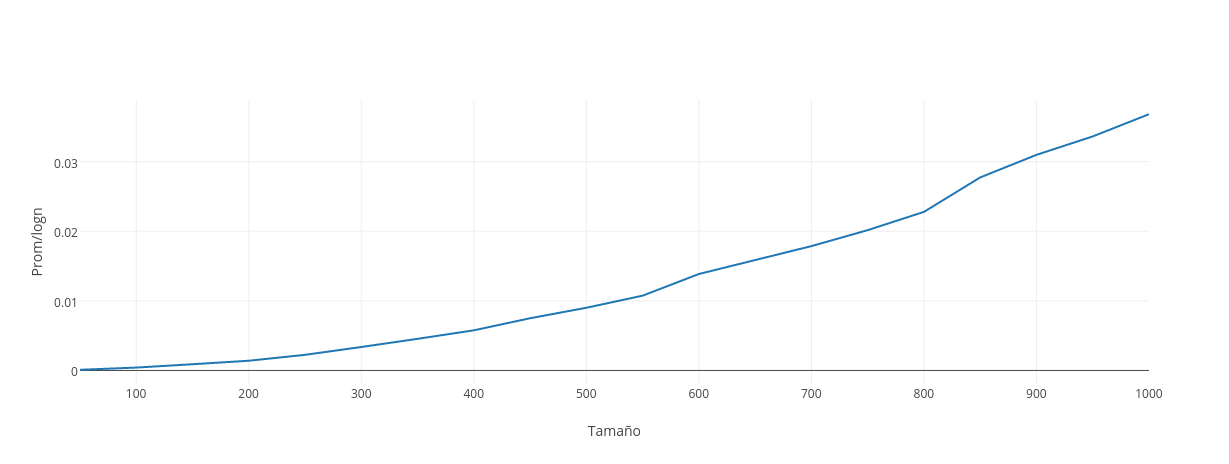
\includegraphics[scale=0.4]{imagenes/ej3/n2.png}
% 	\caption{}
% 	\label{caballito}	
   \end{center}
 \end{figure}
% \newpage

	La morfolog\'ia de este gr\'afico es similar a la anterior, sigue siendo una par\'abola creciente, por lo tanto terminaremos de linealizar, dividiendo a cada uno por $n$, para ver si se trata de la par\'abola cuadr\'atica.\\

   \begin{figure}[h!]
   \begin{center}
 	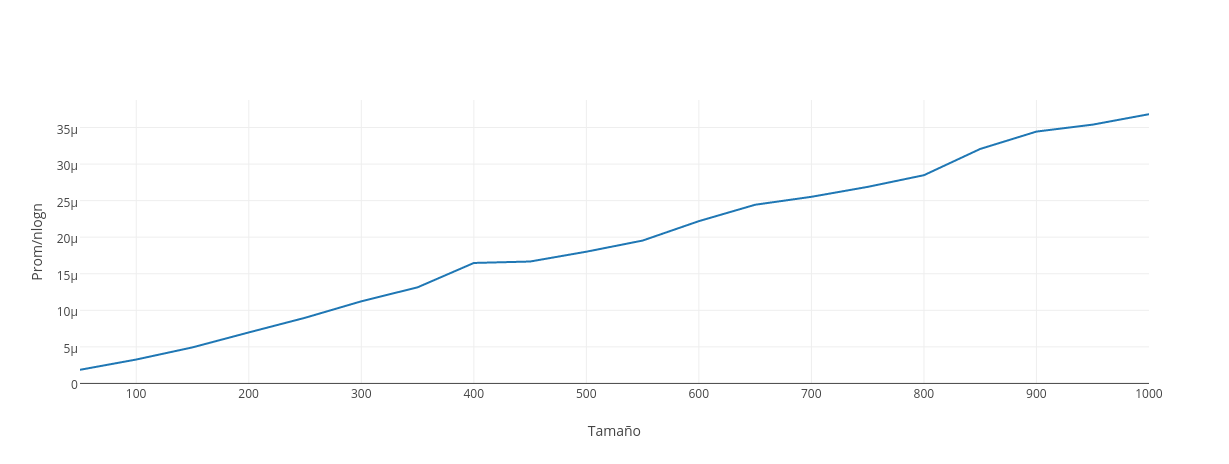
\includegraphics[scale=0.4]{imagenes/ej3/n.png}
% 	\caption{}
% 	\label{caballito}	
   \end{center}
 \end{figure}
% \newpage

	Efectivamente puede observarse que el comportamiento es lineal. Por lo tanto, podemos afirmar que nuestra experimentaci\'on condice a la Cota Te\'orica planteada de $\mathbf{O(n^2.log(n))}$.